\documentclass{article}
    % General document formatting
    \usepackage[margin=0.7in]{geometry}
    \usepackage[parfill]{parskip}
    \usepackage[utf8]{inputenc}
    \usepackage{mathrsfs}
    \usepackage{amsmath}
    \usepackage{amssymb}
    \usepackage{tikz}
    \usepackage{fancyhdr}
    \usepackage{multicol}

    \usetikzlibrary{positioning}

\pagestyle{fancy}
\fancyhf{}
\rhead{Edgar Jacob Rivera Rios - A01184125}

\begin{document}
\section*{2.5.3. Linear Temporal Logic (LTL)}
Prove $\models \neg \diamond \neg p \rightarrow \Box p$ (the converse direction (the sufficiency) of Theorem 13.14 in Ben-Ari, M.).
\begin{align*}
    \models \neg \diamond \neg p &\rightarrow \Box p\\
    \neg \diamond \neg p &= True\\
    \diamond \neg p &= False\\
    \forall s \in S&,\ \forall S_{i} \in \mathscr{I}(s)\\
    S_{i}(P) &= T \equiv \Box p
\end{align*}
\begin{center}
    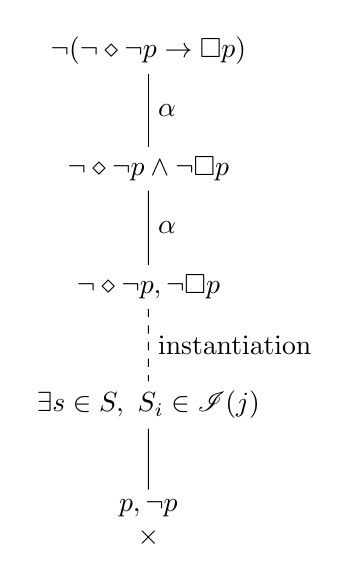
\begin{tikzpicture}[sibling distance=13em, every node/.style = {align=center}]
      \node {$\neg(\neg \diamond \neg p \rightarrow \Box p)$}
        child { node {$\neg \diamond \neg p \wedge \neg \Box p$}
          child {node {$\neg \diamond \neg p, \neg \Box p$}
            child {node {$\exists s \in S,\ S_{i} \in \mathscr{I}(j)$}
              child {node {$p, \neg p$\\$\times$}
              edge from parent [solid] node [right] {}}
            edge from parent [dashed] node [right] {instantiation}}
          edge from parent node [right] {$\alpha$}}
        edge from parent node [right] {$\alpha$}};
    \end{tikzpicture}
\end{center}
\section*{Exercise 2.5.4. Linear Temporal Logic (LTL)}
Prove Theorem 13.15 from Ben-Ari, M.:  $\models \Box (p \rightarrow q) \rightarrow (\Box p \rightarrow \Box q)$.
\begin{align*}
    \models \Box (p \rightarrow q) \rightarrow (\Box p \rightarrow \Box q)\\
    \Box (p \rightarrow q) = True\\
    \forall s \in S,\ \forall S_{i} \in \mathscr{P}(s)
\end{align*}
\begin{center}
    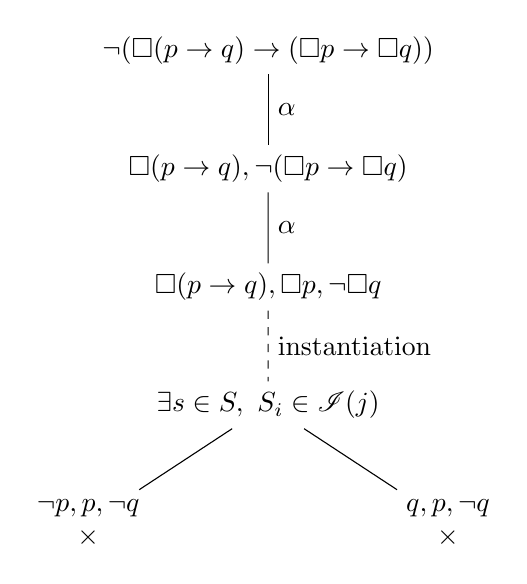
\begin{tikzpicture}[sibling distance=13em, every node/.style = {align=center}]
      \node {$\neg(\Box (p \rightarrow q) \rightarrow (\Box p \rightarrow \Box q))$}
        child { node {$\Box (p \rightarrow q), \neg (\Box p \rightarrow \Box q)$}
          child {node {$\Box (p \rightarrow q), \Box p, \neg \Box q$}
            child {node {$\exists s \in S,\ S_{i} \in \mathscr{I}(j)$}
              child {node {$\neg p, p, \neg q$\\$\times$}
              edge from parent [solid] node [right] {}}
              child {node {$q, p, \neg q$\\$\times$}
              edge from parent [solid] node [right] {}}
            edge from parent [dashed] node [right] {instantiation}}
          edge from parent node [right] {$\alpha$}}
        edge from parent node [right] {$\alpha$}};
    \end{tikzpicture}
\end{center}
\end{document}